\documentclass[11pt,a4paper]{article}

% Packages
\usepackage[utf8]{inputenc}
\usepackage[T1]{fontenc}
\usepackage{geometry}
\usepackage{amsmath,amssymb}
\usepackage{graphicx}
\usepackage{xcolor}
\usepackage{enumitem}
\usepackage{tcolorbox}
\usepackage{tikz}
\usepackage[hidelinks]{hyperref}
\usepackage{fancyhdr}
\usepackage{titlesec}
\usepackage{booktabs}
\usepackage{array}
\usepackage{listings}

% Page geometry
\geometry{margin=1in}

% Colors
\definecolor{questionbg}{RGB}{240,248,255}
\definecolor{answerbg}{RGB}{240,255,240}
\definecolor{reasoningbg}{RGB}{255,250,240}
\definecolor{pytorchcolor}{RGB}{238,76,44}
\definecolor{codegreen}{RGB}{0,128,0}
\definecolor{codegray}{RGB}{128,128,128}
\definecolor{correctbg}{RGB}{200,255,200}

% Code listing style
\lstset{
    basicstyle=\ttfamily\small,
    keywordstyle=\color{pytorchcolor}\bfseries,
    commentstyle=\color{codegray},
    stringstyle=\color{codegreen},
    breaklines=true,
    frame=single,
    backgroundcolor=\color{gray!10}
}

% Custom boxes
\tcbuselibrary{skins,breakable}

\newtcolorbox{questionbox}[1][]{
    colback=questionbg,
    colframe=blue!50!black,
    fonttitle=\bfseries,
    title=#1,
    breakable
}

\newtcolorbox{answerbox}{
    colback=answerbg,
    colframe=green!50!black,
    fonttitle=\bfseries,
    title=Correct Answer,
    breakable
}

\newtcolorbox{reasoningbox}{
    colback=reasoningbg,
    colframe=orange!50!black,
    fonttitle=\bfseries,
    title=Reasoning,
    breakable
}

\newtcolorbox{conceptbox}[1][]{
    colback=gray!10,
    colframe=pytorchcolor,
    fonttitle=\bfseries,
    title=#1,
    breakable
}

% Header/Footer
\pagestyle{fancy}
\fancyhf{}
\fancyhead[L]{\textcolor{pytorchcolor}{\textbf{PyTorch Specialization}}}
\fancyhead[R]{Quiz Study Guide}
\fancyfoot[C]{\thepage}

% Title formatting
\titleformat{\section}{\Large\bfseries\color{pytorchcolor}}{\thesection}{1em}{}
\titleformat{\subsection}{\large\bfseries\color{blue!70!black}}{\thesubsection}{1em}{}

% Correct answer highlight command
\newcommand{\correct}[1]{\colorbox{correctbg}{\textbf{#1}} $\checkmark$}

% Document
\begin{document}

% Title Page
\begin{titlepage}
    \centering
    \vspace*{2cm}
    
    {\Huge\bfseries\color{pytorchcolor} PyTorch Specialization\\[0.5cm]}
    {\LARGE Complete Quiz Study Guide\\[2cm]}
    
    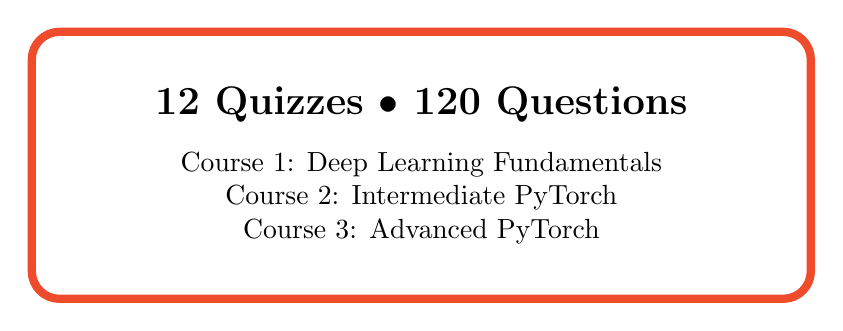
\begin{tikzpicture}
        \node[draw=pytorchcolor, line width=3pt, rounded corners=10pt, inner sep=20pt] {
            \begin{minipage}{0.7\textwidth}
                \centering
                \Large\textbf{12 Quizzes $\bullet$ 120 Questions}\\[0.3cm]
                \normalsize
                Course 1: Deep Learning Fundamentals\\
                Course 2: Intermediate PyTorch\\
                Course 3: Advanced PyTorch
            \end{minipage}
        };
    \end{tikzpicture}
    
    \vfill
    
    {\large All Questions with Options, Answers \& Reasoning}\\[1cm]
    {\large\today}
\end{titlepage}

% Table of Contents
\tableofcontents
\newpage

%==============================================================================
% COURSE 1: DEEP LEARNING FUNDAMENTALS
%==============================================================================
\part{Course 1: Deep Learning Fundamentals}

%------------------------------------------------------------------------------
\section{Quiz 1: PyTorch Basics}
\textit{Topics: Loss Functions, Activation Functions, Epochs, Tensors, Broadcasting}

\begin{questionbox}[Q1]
What does a loss function measure in a neural network?
\end{questionbox}
\begin{answerbox}
The error between predictions and actual values
\end{answerbox}
\begin{reasoningbox}
Loss function quantifies the difference (error) between model predictions and ground truth labels. It provides the signal for optimization - the model adjusts weights to minimize this error.
\end{reasoningbox}

\begin{questionbox}[Q2]
Why do neural networks need non-linear activation functions like ReLU?
\end{questionbox}
\begin{answerbox}
To enable the network to learn non-linear patterns
\end{answerbox}
\begin{reasoningbox}
Without non-linear activations, stacking linear layers results in just another linear transformation (composition of linear functions is linear). ReLU introduces non-linearity, enabling the network to learn complex, non-linear patterns in data.
\end{reasoningbox}

\begin{questionbox}[Q3]
What is an epoch in the context of training neural networks?
\end{questionbox}
\begin{answerbox}
One complete pass through the entire training dataset
\end{answerbox}
\begin{reasoningbox}
An epoch = one full iteration over the entire training dataset. If you have 1000 samples and batch size 100, one epoch = 10 batches. Multiple epochs allow the model to learn from all data repeatedly.
\end{reasoningbox}

\begin{questionbox}[Q4]
What does loss.backward() do in PyTorch?
\end{questionbox}
\begin{answerbox}
Calculates gradients to reduce the loss
\end{answerbox}
\begin{reasoningbox}
loss.backward() performs backpropagation, computing gradients of the loss with respect to all parameters that have requires\_grad=True. These gradients indicate how to adjust weights to reduce the loss.
\end{reasoningbox}

\begin{questionbox}[Q5]
What does dtype specify in a PyTorch tensor?
\end{questionbox}
\begin{answerbox}
The type of numbers stored in the tensor
\end{answerbox}
\begin{reasoningbox}
dtype specifies the data type (float32, float64, int32, int64, etc.) of tensor elements. This affects memory usage, numerical precision, and compatibility with operations.
\end{reasoningbox}

\begin{questionbox}[Q6]
What is the result of: torch.tensor([2., 4., 6.]) / torch.tensor([1., 2., 3.]) + 5?
\end{questionbox}
\begin{answerbox}
tensor([7., 7., 7.])
\end{answerbox}
\begin{reasoningbox}
Element-wise division first: [2/1, 4/2, 6/3] = [2, 2, 2]. Then scalar addition broadcasts: [2+5, 2+5, 2+5] = [7, 7, 7].
\end{reasoningbox}

\begin{questionbox}[Q7]
When you perform operations like multiplication or addition on tensors, what happens?
\end{questionbox}
\begin{answerbox}
Operations apply to each element in the tensor
\end{answerbox}
\begin{reasoningbox}
PyTorch operations are element-wise by default (vectorized operations). This enables efficient parallel computation on GPUs without explicit loops.
\end{reasoningbox}

\begin{questionbox}[Q8]
What makes tensors different from regular Python lists for mathematical operations?
\end{questionbox}
\begin{answerbox}
Tensors are optimized for mathematical operations
\end{answerbox}
\begin{reasoningbox}
Tensors leverage GPU acceleration and optimized C++/CUDA backends for fast math operations. They also support automatic differentiation, broadcasting, and are the fundamental data structure for deep learning.
\end{reasoningbox}

\begin{questionbox}[Q9]
What is the shape of a scalar tensor created by: torch.tensor(5.0).unsqueeze(0).squeeze()?
\end{questionbox}
\begin{answerbox}
torch.Size([])
\end{answerbox}
\begin{reasoningbox}
Starting with scalar (shape []), unsqueeze(0) adds dimension $\rightarrow$ [1], then squeeze() removes ALL size-1 dimensions $\rightarrow$ [] (0-dimensional scalar tensor).
\end{reasoningbox}

\begin{questionbox}[Q10]
What is broadcasting in PyTorch?
\end{questionbox}
\begin{answerbox}
Expanding tensors to compatible shapes for operations
\end{answerbox}
\begin{reasoningbox}
Broadcasting automatically expands smaller tensors to match larger tensor shapes for compatible operations. For example, adding a scalar to a matrix broadcasts the scalar to every element.
\end{reasoningbox}

\newpage
%------------------------------------------------------------------------------
\section{Quiz 2: Training \& Evaluation}
\textit{Topics: Normalization, Model Evaluation, MSE Loss, GPU Setup, Optimizers}

\begin{questionbox}[Q1]
Why do we normalize input data before training a neural network?
\end{questionbox}
\begin{answerbox}
To help the model train more effectively
\end{answerbox}
\begin{reasoningbox}
Normalized data (mean$\approx$0, std$\approx$1) improves gradient flow, prevents vanishing/exploding gradients, and speeds convergence. It ensures all features contribute equally to learning.
\end{reasoningbox}

\begin{questionbox}[Q2]
Why should you use model(x) instead of model.forward(x) for inference?
\end{questionbox}
\begin{answerbox}
Using model() handles PyTorch's internal setup properly
\end{answerbox}
\begin{reasoningbox}
model() invokes \_\_call\_\_() which runs registered hooks, handles nested modules, and calls forward() internally. Directly calling forward() skips these important mechanisms.
\end{reasoningbox}

\begin{questionbox}[Q3]
Why does Mean Squared Error (MSE) square the errors?
\end{questionbox}
\begin{answerbox}
To prevent cancellation and penalize larger errors
\end{answerbox}
\begin{reasoningbox}
Squaring ensures all errors are positive (no cancellation of +/- errors) and disproportionately penalizes larger errors (quadratic penalty). This makes the model focus more on fixing big mistakes.
\end{reasoningbox}

\begin{questionbox}[Q4]
Why do we evaluate models on a separate test set?
\end{questionbox}
\begin{answerbox}
To see if the model learned generalizable patterns
\end{answerbox}
\begin{reasoningbox}
Test set measures generalization to unseen data. Training accuracy alone can mask overfitting - a model might memorize training data but fail on new examples.
\end{reasoningbox}

\begin{questionbox}[Q5]
What is the correct way to set up device for GPU/CPU in PyTorch?
\end{questionbox}
\begin{answerbox}
device = torch.device('cuda' if torch.cuda.is\_available() else 'cpu')
\end{answerbox}
\begin{reasoningbox}
Standard PyTorch idiom: checks CUDA availability, falls back to CPU if no GPU. This makes code portable across different hardware configurations.
\end{reasoningbox}

\begin{questionbox}[Q6]
What does the Flatten layer do in a neural network?
\end{questionbox}
\begin{answerbox}
Reshapes 2D images into 1D vectors
\end{answerbox}
\begin{reasoningbox}
Linear layers expect 1D input. For MNIST, images are 28$\times$28 (2D), so Flatten converts [batch, 1, 28, 28] $\rightarrow$ [batch, 784] for the fully connected layers.
\end{reasoningbox}

\begin{questionbox}[Q7]
Which optimizer is generally recommended as a good default choice?
\end{questionbox}
\begin{answerbox}
Adam
\end{answerbox}
\begin{reasoningbox}
Adam combines momentum + adaptive learning rates (per-parameter). It works well across diverse problems without much hyperparameter tuning, making it an excellent default choice.
\end{reasoningbox}

\begin{questionbox}[Q8]
Should you shuffle data in DataLoader for training and testing?
\end{questionbox}
\begin{answerbox}
Shuffle training data, but not test data
\end{answerbox}
\begin{reasoningbox}
Shuffling training data prevents learning order-dependent patterns and ensures varied batches. Test order doesn't affect metric computation, and keeping it fixed aids reproducibility.
\end{reasoningbox}

\begin{questionbox}[Q9]
What does torch.no\_grad() do?
\end{questionbox}
\begin{answerbox}
Disables gradient tracking to save memory
\end{answerbox}
\begin{reasoningbox}
torch.no\_grad() disables autograd gradient computation, reducing memory usage and speeding up inference. Used during evaluation when gradients aren't needed.
\end{reasoningbox}

\begin{questionbox}[Q10]
What does model.eval() do?
\end{questionbox}
\begin{answerbox}
Changes how certain layers behave during evaluation
\end{answerbox}
\begin{reasoningbox}
model.eval() switches layers like Dropout (disabled) and BatchNorm (uses running statistics instead of batch statistics) to evaluation behavior. Always use before inference.
\end{reasoningbox}

\newpage
%------------------------------------------------------------------------------
\section{Quiz 3: Data Pipelines}
\textit{Topics: Custom Datasets, DataLoader, Transforms, Data Augmentation}

\begin{questionbox}[Q1]
In the lecture, why did three different teams building the flower identification app get such different results even though they used the same model architecture?
\begin{enumerate}[label=\Alph*.]
    \item They trained for different numbers of epochs
    \item \correct{They handled and prepared the data differently}
    \item They used different batch sizes
    \item They used different loss functions
\end{enumerate}
\end{questionbox}
\begin{reasoningbox}
Data preparation (preprocessing, augmentation, splitting) has huge impact on model performance, even with identical architectures. The same model can succeed or fail based purely on data handling.
\end{reasoningbox}

\begin{questionbox}[Q2]
Three categories of data pipeline problems are introduced: access, quality, and efficiency. Which category involves loading data in batches rather than one item at a time?
\begin{enumerate}[label=\Alph*.]
    \item Quality problems
    \item Architecture problems
    \item \correct{Efficiency problems}
    \item Access problems
\end{enumerate}
\end{questionbox}
\begin{reasoningbox}
Loading data in batches rather than one at a time is an efficiency optimization to speed up training. Batching enables parallel processing and better GPU utilization.
\end{reasoningbox}

\begin{questionbox}[Q3]
In the \_\_init\_\_ method of the Oxford Flowers dataset, why are image paths stored but the actual images not loaded into memory?
\begin{enumerate}[label=\Alph*.]
    \item Images must be transformed before loading
    \item PyTorch doesn't allow loading images in \_\_init\_\_
    \item Loading images in \_\_init\_\_ would be too slow
    \item \correct{Loading all images at once would use too much memory}
\end{enumerate}
\end{questionbox}
\begin{reasoningbox}
Storing paths in \_\_init\_\_ and loading images lazily in \_\_getitem\_\_ prevents memory overflow with large datasets. This is the standard lazy loading pattern for efficient data handling.
\end{reasoningbox}

\begin{questionbox}[Q4]
The Oxford Flowers dataset labels range from 1 to 102, but PyTorch expects labels from 0 to 101. Where should you fix this indexing issue?
\begin{enumerate}[label=\Alph*.]
    \item \correct{In the \_\_init\_\_ method by subtracting 1 from all labels}
    \item In the \_\_getitem\_\_ method when returning each label
    \item PyTorch will automatically adjust the labels
    \item In the \_\_len\_\_ method when reporting dataset size
\end{enumerate}
\end{questionbox}
\begin{reasoningbox}
Fix indexing in \_\_init\_\_ by subtracting 1 from all labels \textbf{once}, rather than in \_\_getitem\_\_ which runs thousands of times during training. This is more efficient.
\end{reasoningbox}

\begin{questionbox}[Q5]
Why does the Normalize transform help neural networks learn more effectively?
\begin{enumerate}[label=\Alph*.]
    \item \correct{It spreads pixel values for better gradient-based learning}
    \item It reduces the file size of images
    \item It converts images from PIL format to tensors
    \item It makes all images the same brightness
\end{enumerate}
\end{questionbox}
\begin{reasoningbox}
Normalize centers data around 0 with unit variance, spreading values optimally for gradient-based optimization. This improves gradient flow and training stability.
\end{reasoningbox}

\begin{questionbox}[Q6]
ToTensor() performs three important operations. Which of the following is NOT one of them?
\begin{enumerate}[label=\Alph*.]
    \item \correct{Normalizes pixel values using mean and standard deviation}
    \item Converts the image from a PIL object to a PyTorch tensor
    \item Scales pixel values from 0-255 to 0-1
    \item Rearranges dimensions to [channels, height, width]
\end{enumerate}
\end{questionbox}
\begin{reasoningbox}
ToTensor() does: PIL$\rightarrow$tensor, scales 0-255$\rightarrow$0-1, rearranges to [C,H,W]. Mean/std normalization is a \textbf{separate} Normalize() transform that must be applied explicitly.
\end{reasoningbox}

\begin{questionbox}[Q7]
What's wrong with loading data from a large file inside the \_\_getitem\_\_ method instead of in \_\_init\_\_?
\begin{enumerate}[label=\Alph*.]
    \item It prevents the DataLoader from shuffling the data
    \item It causes the data to be loaded into memory all at once and crash
    \item \correct{The entire file is read for every sample access}
    \item PyTorch doesn't allow file reading in \_\_getitem\_\_
\end{enumerate}
\end{questionbox}
\begin{reasoningbox}
Reading from a large file in \_\_getitem\_\_ may re-read/re-parse the entire file for each sample access—extremely inefficient. Load metadata once in \_\_init\_\_, access individual items in \_\_getitem\_\_.
\end{reasoningbox}

\begin{questionbox}[Q8]
When you iterate through a DataLoader, what does each iteration give you?
\begin{enumerate}[label=\Alph*.]
    \item \correct{A batch of images and a batch of labels}
    \item A single image and its label
    \item Just the images—you need to fetch labels separately
    \item The entire dataset at once
\end{enumerate}
\end{questionbox}
\begin{reasoningbox}
DataLoader returns batched tensors: a batch of inputs and a batch of corresponding labels together. This is the standard pattern for training loops.
\end{reasoningbox}

\begin{questionbox}[Q9]
Why should you apply data augmentation to the training set but not to the validation set?
\begin{enumerate}[label=\Alph*.]
    \item PyTorch doesn't support augmentation on validation data
    \item Augmentation only works on images the model has already seen
    \item \correct{Validation needs consistent data to measure improvements reliably}
    \item Augmentation is too slow to apply during validation
\end{enumerate}
\end{questionbox}
\begin{reasoningbox}
Augmentation adds randomness for training diversity; validation data should be consistent across epochs to reliably measure model improvement. Random validation would give noisy metrics.
\end{reasoningbox}

\begin{questionbox}[Q10]
In the robust dataset implementation, what happens when \_\_getitem\_\_ encounters a corrupted or problematic image?
\begin{enumerate}[label=\Alph*.]
    \item \correct{It logs the error and retrieves another valid image}
    \item It returns None and continues to the next batch
    \item It raises an exception and stops training
    \item It replaces the corrupted image with a blank tensor
\end{enumerate}
\end{questionbox}
\begin{reasoningbox}
A robust implementation catches exceptions and returns a different valid sample to keep training going without crashing. This handles real-world data quality issues gracefully.
\end{reasoningbox}

\newpage
%------------------------------------------------------------------------------
\section{Quiz 4: CNNs \& Model Architecture}
\textit{Topics: Convolutional Layers, Pooling, nn.Module, nn.Sequential}

\begin{questionbox}[Q1]
What is the key advantage of having CNNs learn their own filters rather than using hand-designed filters?
\begin{enumerate}[label=\Alph*.]
    \item Hand-designed filters need extra storage for configuration metadata
    \item Learned filters work for any image classification task without retraining
    \item \correct{The model discovers task-specific patterns automatically}
    \item Hand-designed filters are too slow to compute
\end{enumerate}
\end{questionbox}
\begin{reasoningbox}
Learned filters adapt to the specific task, automatically discovering optimal patterns for that dataset rather than relying on generic hand-designed features like edge detectors.
\end{reasoningbox}

\begin{questionbox}[Q2]
What is the sequence of operations that happens when a filter performs a convolution at one position in an image?
\begin{enumerate}[label=\Alph*.]
    \item Multiply all pixel values together, then add the filter values
    \item Add filter values to pixel values, then multiply, then average
    \item \correct{Multiply corresponding values element-wise, then sum the products}
    \item Average the pixel values first, then multiply by the filter
\end{enumerate}
\end{questionbox}
\begin{reasoningbox}
Convolution operation: element-wise multiply filter values with corresponding pixel values in the receptive field, then sum all the products to get one output value.
\end{reasoningbox}

\begin{questionbox}[Q3]
A CNN has two convolutional layers, each followed by MaxPool2d with kernel\_size=2. If the input image is 28$\times$28 pixels, what size are the feature maps after both pooling layers?
\begin{enumerate}[label=\Alph*.]
    \item \correct{7$\times$7}
    \item 14$\times$14
    \item 3$\times$3
    \item 28$\times$28
\end{enumerate}
\end{questionbox}
\begin{reasoningbox}
$28\times28 \xrightarrow{\text{MaxPool(2)}} 14\times14 \xrightarrow{\text{MaxPool(2)}} 7\times7$. Each MaxPool with kernel=2 halves the spatial dimensions.
\end{reasoningbox}

\begin{questionbox}[Q4]
In a convolutional layer with in\_channels=3 and out\_channels=32, what does the 32 represent?
\begin{enumerate}[label=\Alph*.]
    \item The layer processes 32 images at once in a batch
    \item The output image will be 32$\times$32 pixels
    \item \correct{The layer learns 32 different filters}
    \item The layer creates 32 copies of each input channel
\end{enumerate}
\end{questionbox}
\begin{reasoningbox}
out\_channels=32 means the layer learns 32 separate filters, each producing one output feature map. Each filter detects a different pattern.
\end{reasoningbox}

\begin{questionbox}[Q5]
What is a key limitation of using nn.Sequential to define a model in PyTorch?
\begin{enumerate}[label=\Alph*.]
    \item \correct{Sequential doesn't support conditionals, loops, or branching}
    \item Sequential cannot be used with the Adam optimizer
    \item Sequential models train slower than models using nn.Module
    \item Sequential models cannot use convolutional layers
\end{enumerate}
\end{questionbox}
\begin{reasoningbox}
nn.Sequential is a simple linear stack of layers. For conditionals, loops, or branching architectures (like ResNet skip connections), you must subclass nn.Module and define custom forward().
\end{reasoningbox}

\begin{questionbox}[Q6]
What is the core difference between how static graphs and PyTorch's dynamic graphs work?
\begin{enumerate}[label=\Alph*.]
    \item Static graphs require defining everything in one block while dynamic graphs split definitions across methods
    \item Static graphs run faster but dynamic graphs use less memory
    \item Static graphs only work with images while dynamic graphs work with any data type
    \item \correct{Static graphs are defined once before training, while dynamic graphs are built fresh each forward pass}
\end{enumerate}
\end{questionbox}
\begin{reasoningbox}
PyTorch uses dynamic graphs rebuilt on each forward pass, unlike static graphs (TensorFlow 1.x style) defined once before execution. This enables flexible architectures with conditionals and loops.
\end{reasoningbox}

\begin{questionbox}[Q7]
Why does PyTorch separate the \_\_init\_\_ and forward methods instead of combining them into a single method?
\begin{enumerate}[label=\Alph*.]
    \item The \_\_init\_\_ method runs faster than the forward method
    \item \correct{\_\_init\_\_ defines the architecture, forward defines how data flows through it}
    \item It makes the code easier to read by splitting it into smaller sections
    \item It's a Python convention that all classes must follow
\end{enumerate}
\end{questionbox}
\begin{reasoningbox}
\_\_init\_\_ creates and initializes layers (architecture definition), forward() defines how input data flows through those layers (computation graph). Separation enables flexible, dynamic architectures.
\end{reasoningbox}

\begin{questionbox}[Q8]
When defining a custom nn.Module, what is one benefit of using nn.Sequential to organize its layers?
\begin{enumerate}[label=\Alph*.]
    \item Sequential automatically chooses the best layer order for your data
    \item Sequential allows you to use conditionals and loops in your model
    \item \correct{You don't need to manually call each layer in forward()}
    \item Sequential makes the model train faster
\end{enumerate}
\end{questionbox}
\begin{reasoningbox}
nn.Sequential automatically chains layer calls in order, so you just call self.features(x) instead of manually calling each layer: conv1, relu1, pool1, conv2, etc.
\end{reasoningbox}

\begin{questionbox}[Q9]
What is the standard way to count the total number of parameters in a PyTorch model?
\begin{enumerate}[label=\Alph*.]
    \item print(model.parameters())
    \item model.count\_parameters()
    \item len(model.parameters())
    \item \correct{sum(p.numel() for p in model.parameters())}
\end{enumerate}
\end{questionbox}
\begin{reasoningbox}
model.parameters() returns an iterator of parameter tensors; p.numel() gives element count per tensor; sum() totals all elements across all parameters.
\end{reasoningbox}

\begin{questionbox}[Q10]
What is the key difference between model.children() and model.modules() when inspecting a PyTorch model?
\begin{enumerate}[label=\Alph*.]
    \item children() is faster but modules() is more detailed
    \item \correct{children() shows only direct children, modules() shows all nested modules recursively}
    \item modules() only works with Sequential blocks while children() works with all layers
    \item children() shows parameters while modules() shows layers
\end{enumerate}
\end{questionbox}
\begin{reasoningbox}
children() returns only immediate child modules (one level); modules() recursively returns ALL nested modules including the model itself and deeply nested layers.
\end{reasoningbox}

\newpage
%==============================================================================
% COURSE 2: INTERMEDIATE PYTORCH
%==============================================================================
\part{Course 2: Intermediate PyTorch}

%------------------------------------------------------------------------------
\section{Quiz 5: Hyperparameter Optimization (Optuna)}
\textit{Topics: Flexible CNN, Parameter Importance, Model Selection}

\begin{questionbox}[Q1]
Which of the following best describes the design principle behind parameterizing a model architecture for use with tools like Optuna?
\begin{enumerate}[label=\Alph*.]
    \item It ensures Optuna trials are deterministic by locking random seeds
    \item It simplifies the forward pass logic in PyTorch's nn.Module
    \item \correct{It supports flexible experimentation by testing multiple architectural designs}
    \item It enforces model reproducibility through fixed layer structures
\end{enumerate}
\end{questionbox}
\begin{reasoningbox}
Parameterizing architecture allows Optuna to systematically explore different configurations (number of layers, layer sizes, dropout rates) for flexible experimentation and automated architecture search.
\end{reasoningbox}

\begin{questionbox}[Q2]
True or False: Both dropout rate and learning rate are regularization hyperparameters.
\begin{enumerate}[label=\Alph*.]
    \item \correct{False}
    \item True
\end{enumerate}
\end{questionbox}
\begin{reasoningbox}
Dropout is a regularization technique (prevents overfitting by randomly dropping neurons). Learning rate is an \textbf{optimization} hyperparameter that controls step size during gradient descent—not regularization.
\end{reasoningbox}

\begin{questionbox}[Q3]
Complete the code to allow dynamic dropout selection between 0.1 and 0.5:
\begin{lstlisting}[language=Python]
def objective(trial):
    n_layers = trial.suggest_int("n_layers", 1, 3)
    fc_size = trial.suggest_int("fc_size", 64, 512, step=64)
    # What goes here?
\end{lstlisting}
\begin{enumerate}[label=\Alph*.]
    \item dropout\_rate = trial.sample\_float("dropout\_rate", 0.1, 0.5)
    \item dropout\_rate = FlexibleCNN.suggest("dropout\_rate", 0.1, 0.5)
    \item \correct{dropout\_rate = trial.suggest\_float("dropout\_rate", 0.1, 0.5)}
    \item dropout\_rate = trial.suggest\_categorical("dropout\_rate", [0.1, 0.2, 0.3, 0.4, 0.5])
\end{enumerate}
\end{questionbox}
\begin{reasoningbox}
suggest\_float() is for continuous float ranges in Optuna. suggest\_categorical would only give discrete predefined values; sample\_float is not a valid method.
\end{reasoningbox}

\begin{questionbox}[Q4]
Which of the following is a best practice when designing an optimization pipeline using Optuna?
\begin{enumerate}[label=\Alph*.]
    \item Define all hyperparameters regardless of their dependencies
    \item \correct{Structure the search space to reflect dependencies between architectural components}
    \item Include only training hyperparameters like learning rate and batch size
    \item Test all possible combinations of hyperparameters exhaustively
\end{enumerate}
\end{questionbox}
\begin{reasoningbox}
Best practice: only define hyperparameters for components that exist in that trial configuration (conditional search space). For example, don't tune layer 3's size if n\_layers=2.
\end{reasoningbox}

\begin{questionbox}[Q5]
Why might you prioritize evaluating model size and inference time in addition to accuracy?
\begin{enumerate}[label=\Alph*.]
    \item To better understand the GPU temperature behavior
    \item These values are easier to measure than accuracy
    \item \correct{To ensure your model meets real-world deployment constraints like speed and memory}
    \item Accuracy always guarantees generalization anyway
\end{enumerate}
\end{questionbox}
\begin{reasoningbox}
Real-world deployment has practical constraints: latency requirements, memory limits, edge device capabilities. A highly accurate but slow/large model may be unusable in production.
\end{reasoningbox}

\begin{questionbox}[Q6]
Why is the classifier initialized inside the forward method in a flexible CNN architecture?
\begin{enumerate}[label=\Alph*.]
    \item To reset the classifier weights every forward pass
    \item To delay initialization until the model is fully trained
    \item \correct{Because x.size(1) gives the dynamic flattened feature size, which depends on earlier layers}
    \item To prevent the classifier from being saved in the model checkpoint
\end{enumerate}
\end{questionbox}
\begin{reasoningbox}
Classifier input size depends on the dynamic architecture (number of conv layers, kernel sizes, pooling). The flattened feature size is only known after running the convolutional layers, so lazy initialization is needed.
\end{reasoningbox}

\begin{questionbox}[Q7]
What insight can you gain by analyzing parameter importances after an Optuna optimization run?
\begin{enumerate}[label=\Alph*.]
    \item You can identify which training samples contributed most to performance
    \item \correct{You can determine which hyperparameters had the most influence on the objective}
    \item You can determine the exact optimal hyperparameter combination
    \item You can identify which hyperparameters caused underfitting
\end{enumerate}
\end{questionbox}
\begin{reasoningbox}
Parameter importance analysis reveals which hyperparameters most influence the objective function. This helps prioritize future search efforts on the most impactful parameters.
\end{reasoningbox}

\begin{questionbox}[Q8]
How does the parallel coordinate plot help in understanding the results of a hyperparameter search?
\begin{enumerate}[label=\Alph*.]
    \item It shows epoch-wise performance trends
    \item It plots validation loss across models
    \item \correct{It highlights optimal combinations of hyperparameter values using color intensity}
    \item It ranks models based on final test accuracy
\end{enumerate}
\end{questionbox}
\begin{reasoningbox}
Parallel coordinate plots show lines connecting hyperparameter values across axes, with color intensity indicating performance quality. You can visually identify which value combinations lead to good results.
\end{reasoningbox}

\begin{questionbox}[Q9]
In a hyperparameter tuning process, what is the primary role of a baseline model?
\begin{enumerate}[label=\Alph*.]
    \item To automate model selection based on predefined criteria
    \item \correct{To serve as a reference point against which performance improvements can be measured}
    \item To maximize model complexity during early experimentation
    \item To confirm that your model is generalizing well to new data
\end{enumerate}
\end{questionbox}
\begin{reasoningbox}
A baseline model provides a reference point to quantify whether optimized models actually improve performance. Without a baseline, you can't tell if your tuning efforts are helping.
\end{reasoningbox}

\begin{questionbox}[Q10]
Given the formula Score = 0.5 $\times$ Accuracy + 0.3 $\times$ Memory + 0.2 $\times$ Time, and these normalized metrics:
\begin{center}
\begin{tabular}{lccc}
\toprule
Model & Accuracy & Memory & Time \\
\midrule
A & 0.8 & 0.7 & 0.3 \\
B & 0.6 & 0.7 & 0.9 \\
C & 0.7 & 0.6 & 0.95 \\
D & 0.75 & 0.8 & 0.2 \\
\bottomrule
\end{tabular}
\end{center}
Which model wins?
\begin{enumerate}[label=\Alph*.]
    \item \correct{C}
    \item D
    \item B
    \item A
\end{enumerate}
\end{questionbox}
\begin{reasoningbox}
Calculate scores: A = 0.5(0.8)+0.3(0.7)+0.2(0.3) = 0.67. B = 0.5(0.6)+0.3(0.7)+0.2(0.9) = 0.69. \textbf{C = 0.5(0.7)+0.3(0.6)+0.2(0.95) = 0.72}. D = 0.5(0.75)+0.3(0.8)+0.2(0.2) = 0.655. Model C has the highest score.
\end{reasoningbox}

\newpage
%------------------------------------------------------------------------------
\section{Quiz 6: TorchVision \& Transfer Learning}
\textit{Topics: PIL, Transforms, Pretrained Models, Semantic Segmentation}

\begin{questionbox}[Q1]
What is one key advantage of using domain-specific libraries like TorchVision for vision tasks?
\begin{enumerate}[label=\Alph*.]
    \item \correct{They offer optimized tools, datasets, and pretrained models tailored for vision workflows}
    \item They provide generic tools applicable to any data type
    \item They eliminate the need for training models entirely
    \item They automatically improve accuracy of any model
\end{enumerate}
\end{questionbox}
\begin{reasoningbox}
Domain-specific libraries like TorchVision provide specialized, optimized tools (transforms, datasets, pretrained models) specifically designed for vision tasks, saving development time and ensuring best practices.
\end{reasoningbox}

\begin{questionbox}[Q2]
Which library does TorchVision rely on for image file I/O and manipulation before tensor conversion?
\begin{enumerate}[label=\Alph*.]
    \item seaborn
    \item NumPy
    \item \correct{PIL (Pillow)}
    \item OpenCV
\end{enumerate}
\end{questionbox}
\begin{reasoningbox}
TorchVision relies on PIL (Pillow) for image I/O and manipulation before converting images to tensors. PIL is the standard Python imaging library integrated with TorchVision transforms.
\end{reasoningbox}

\begin{questionbox}[Q3]
What is the primary goal of transfer learning?
\begin{enumerate}[label=\Alph*.]
    \item To combine multiple model architectures into a single ensemble
    \item To reduce the computational cost of inference only
    \item \correct{To leverage knowledge gained from pre-training on large datasets}
    \item To train models from scratch more efficiently
\end{enumerate}
\end{questionbox}
\begin{reasoningbox}
Transfer learning leverages pretrained weights from large datasets (like ImageNet) to jumpstart learning on new tasks with less data. The model transfers learned features to the new domain.
\end{reasoningbox}

\begin{questionbox}[Q4]
What will draw\_bounding\_boxes() do when called?
\begin{enumerate}[label=\Alph*.]
    \item It runs object detection and returns the predicted boxes
    \item \correct{It returns a new image tensor with boxes and labels drawn on it}
    \item It modifies the original image tensor in place
    \item It saves the image with bounding boxes to disk
\end{enumerate}
\end{questionbox}
\begin{reasoningbox}
draw\_bounding\_boxes() returns a NEW tensor with boxes/labels drawn; it doesn't modify in-place, run detection, or save to disk. It's purely a visualization utility.
\end{reasoningbox}

\begin{questionbox}[Q5]
Why would you apply RandomResizedCrop() instead of just RandomCrop()?
\begin{enumerate}[label=\Alph*.]
    \item To ensure all crops are center-aligned after resizing
    \item To crop images at a random location but with a fixed aspect ratio
    \item To normalize pixel intensity ranges after cropping
    \item \correct{To introduce random cropping along with random resizing, simulating scale variation}
\end{enumerate}
\end{questionbox}
\begin{reasoningbox}
RandomResizedCrop applies random scale changes AND random cropping, simulating objects appearing at different sizes/distances. This is powerful data augmentation for scale invariance.
\end{reasoningbox}

\begin{questionbox}[Q6]
Why is it important to apply Resize() before CenterCrop() or RandomCrop()?
\begin{enumerate}[label=\Alph*.]
    \item To convert the image to grayscale first
    \item \correct{To ensure the image is large enough to safely crop to the target size}
    \item To change the image color depth
    \item To remove background artifacts before cropping
\end{enumerate}
\end{questionbox}
\begin{reasoningbox}
Resize ensures image dimensions are $\geq$ crop size. Cropping an image smaller than the target size would fail or produce unexpected results.
\end{reasoningbox}

\begin{questionbox}[Q7]
Where should Normalize() typically be applied in an image transform pipeline?
\begin{enumerate}[label=\Alph*.]
    \item Before converting the image to a tensor
    \item Before loading the image from disk
    \item \correct{Immediately after converting to a tensor with ToTensor()}
    \item After training is complete
\end{enumerate}
\end{questionbox}
\begin{reasoningbox}
Normalize requires tensor input (operates on float tensors), so it must come after ToTensor() in the transform pipeline. ToTensor first, then Normalize.
\end{reasoningbox}

\begin{questionbox}[Q8]
What output does a pretrained DeepLabV3 semantic segmentation model produce?
\begin{enumerate}[label=\Alph*.]
    \item A tensor of class scores for the entire image
    \item A single prediction of what class is in the image
    \item A list of bounding boxes around detected objects
    \item \correct{A per-pixel tensor indicating the predicted class for each pixel}
\end{enumerate}
\end{questionbox}
\begin{reasoningbox}
DeepLabV3 is a semantic segmentation model outputting per-pixel class predictions—a dense prediction where every pixel gets classified (not bounding boxes or single class).
\end{reasoningbox}

\begin{questionbox}[Q9]
Fill in the missing transform for using a pretrained segmentation model:
\begin{lstlisting}[language=Python]
transform = transforms.Compose([
    transforms.ToTensor(),
    ___________
])
\end{lstlisting}
\begin{enumerate}[label=\Alph*.]
    \item \correct{transforms.Normalize([0.485, 0.456, 0.406], [0.229, 0.224, 0.225])}
    \item transforms.CenterCrop(224)
    \item transforms.Grayscale()
    \item transforms.Resize((32, 32))
\end{enumerate}
\end{questionbox}
\begin{reasoningbox}
Pretrained models expect ImageNet normalization: mean=[0.485, 0.456, 0.406], std=[0.229, 0.224, 0.225]. This matches the preprocessing used during original training.
\end{reasoningbox}

\begin{questionbox}[Q10]
Why is unsqueeze(0) often used after converting an image to a tensor for model input?
\begin{enumerate}[label=\Alph*.]
    \item \correct{It adds a batch dimension so the input shape is [1, C, H, W]}
    \item It adds a color channel to grayscale images
    \item It flattens the image for matrix multiplication
    \item It ensures the pixel values are between 0 and 1
\end{enumerate}
\end{questionbox}
\begin{reasoningbox}
Models expect 4D input [batch, channels, height, width]. unsqueeze(0) adds the batch dimension to transform a single image from [C,H,W] to [1,C,H,W].
\end{reasoningbox}

\newpage
%------------------------------------------------------------------------------
\section{Quiz 7: NLP Fundamentals}
\textit{Topics: Tokenization, Embeddings, BERT, Padding, OOV, NER}

\begin{questionbox}[Q1]
Why is lowercasing commonly applied during manual tokenization in NLP preprocessing?
\begin{enumerate}[label=\Alph*.]
    \item \correct{To reduce vocabulary size by treating "Word" and "word" as the same token}
    \item To improve model precision on named entities
    \item To encode sentiment information in the text
    \item To truncate long tokens to a maximum length
\end{enumerate}
\end{questionbox}
\begin{reasoningbox}
Lowercasing merges "Word", "WORD", "word" into a single token, reducing vocabulary size and sparsity. This simplifies the model but may lose case-based information (proper nouns, acronyms).
\end{reasoningbox}

\begin{questionbox}[Q2]
When using nn.EmbeddingBag instead of nn.Embedding, what key advantage does it provide?
\begin{enumerate}[label=\Alph*.]
    \item \correct{It automatically pools (sums/means) embeddings across tokens in one operation}
    \item It eliminates the need for tokenization entirely
    \item It supports static but not dynamic embeddings
    \item It automatically generates attention masks
\end{enumerate}
\end{questionbox}
\begin{reasoningbox}
nn.EmbeddingBag computes sum/mean of embeddings in one efficient operation, vs separate embedding lookup + pooling steps. Useful for bag-of-words style representations.
\end{reasoningbox}

\begin{questionbox}[Q3]
What is the main purpose of padding sequences in a batch for NLP?
\begin{enumerate}[label=\Alph*.]
    \item \correct{To ensure all sequences in a batch have the same length for tensor operations}
    \item To convert words into one-hot vectors
    \item To remove irrelevant tokens from sequences
    \item To truncate sequences that are too long
\end{enumerate}
\end{questionbox}
\begin{reasoningbox}
Batched tensor operations require uniform dimensions. Padding ensures all sequences have the same length so they can be stacked into a single tensor for parallel processing.
\end{reasoningbox}

\begin{questionbox}[Q4]
When using pretrained embeddings, why would you "freeze" the embedding weights?
\begin{enumerate}[label=\Alph*.]
    \item To improve tokenizer efficiency
    \item To automatically generate attention masks
    \item \correct{To prevent gradient updates and retain the pretrained semantic representations}
    \item To reduce GPU memory usage during inference only
\end{enumerate}
\end{questionbox}
\begin{reasoningbox}
Freezing embedding weights (requires\_grad=False) prevents gradient updates, preserving the learned semantic knowledge from large-scale pretraining. Useful when you have limited data.
\end{reasoningbox}

\begin{questionbox}[Q5]
Which is NOT a typical preprocessing step before sending input to a pretrained BERT model?
\begin{enumerate}[label=\Alph*.]
    \item Lowercasing text (for uncased models)
    \item Tokenizing into subwords or word pieces
    \item Padding sequences to a uniform length
    \item \correct{Converting token IDs back into strings}
\end{enumerate}
\end{questionbox}
\begin{reasoningbox}
Preprocessing converts strings TO tokens/IDs for model input. Converting tokens back to strings is the reverse operation (decoding output), not preprocessing.
\end{reasoningbox}

\begin{questionbox}[Q6]
Which method is commonly used to handle Out Of Vocabulary (OOV) words?
\begin{enumerate}[label=\Alph*.]
    \item Dropping all OOV words from the dataset entirely
    \item \correct{Using subword tokenization (BPE, WordPiece) to break unknown words into known pieces}
    \item Using rule-based systems to manually define meanings
    \item Simply ignoring the issue during training
\end{enumerate}
\end{questionbox}
\begin{reasoningbox}
Subword tokenization (BPE, WordPiece) handles OOV by breaking unknown words into known subword units. Even unseen words can be represented as combinations of known pieces, plus [UNK] as fallback.
\end{reasoningbox}

\begin{questionbox}[Q7]
What happens when you apply a BERT tokenizer with padding=True, truncation=True, return\_tensors="pt"?
\begin{enumerate}[label=\Alph*.]
    \item It converts text into character-level tensors
    \item It automatically trains a model on the input
    \item \correct{It outputs PyTorch tensors with padded/truncated input\_ids and attention\_mask}
    \item It removes all unknown tokens entirely from the input
\end{enumerate}
\end{questionbox}
\begin{reasoningbox}
BERT tokenizer with those arguments returns a dictionary with input\_ids and attention\_mask as PyTorch tensors, properly padded to uniform length and truncated if too long.
\end{reasoningbox}

\begin{questionbox}[Q8]
What is the purpose of nn.Embedding in a text classifier?
\begin{enumerate}[label=\Alph*.]
    \item It directly predicts class probabilities from token indices
    \item \correct{It maps discrete token indices to dense vectors that capture semantic similarity}
    \item It normalizes embeddings to unit vectors automatically
    \item It applies padding and truncation to input sequences
\end{enumerate}
\end{questionbox}
\begin{reasoningbox}
nn.Embedding maps discrete token indices to continuous dense vectors in a semantic space where similar words are closer together. It's a learnable lookup table.
\end{reasoningbox}

\begin{questionbox}[Q9]
What is Named Entity Recognition (NER)?
\begin{enumerate}[label=\Alph*.]
    \item A system that evaluates sentiment polarity in text
    \item A method to generate abstractive text summaries
    \item A technique for translating text between languages
    \item \correct{A process that identifies and classifies entities like people, organizations, and locations}
\end{enumerate}
\end{questionbox}
\begin{reasoningbox}
NER (Named Entity Recognition) identifies and classifies named entities in text into predefined categories: PERSON, ORGANIZATION, LOCATION, DATE, etc.
\end{reasoningbox}

\begin{questionbox}[Q10]
What key aspect should you consider when selecting pretrained word embeddings for your task?
\begin{enumerate}[label=\Alph*.]
    \item \correct{Vocabulary size and domain coverage}
    \item Training batch size used originally
    \item Number of epochs in original training
    \item Total training duration in hours
\end{enumerate}
\end{questionbox}
\begin{reasoningbox}
Vocabulary coverage is critical for pretrained embeddings. Domain mismatch (e.g., medical text with general embeddings) leads to high OOV rates and poor performance.
\end{reasoningbox}

\newpage
%------------------------------------------------------------------------------
\section{Quiz 8: Performance Optimization}
\textit{Topics: DataLoader, Profiler, Mixed Precision, Gradient Accumulation, Lightning}

\begin{questionbox}[Q1]
What is the main goal when optimizing batch size in DataLoader?
\begin{enumerate}[label=\Alph*.]
    \item Always use the largest possible batch size
    \item Set batch size equal to the number of DataLoader workers
    \item \correct{Find a balance that maximizes GPU utilization while fitting within memory limits}
    \item Use the smallest batch size to reduce memory usage
\end{enumerate}
\end{questionbox}
\begin{reasoningbox}
Batch size optimization balances GPU utilization (larger = better parallelism) against memory limits (too large = OOM error). Find the sweet spot for your hardware.
\end{reasoningbox}

\begin{questionbox}[Q2]
What is pinned memory in PyTorch DataLoader?
\begin{enumerate}[label=\Alph*.]
    \item Memory that is shared between CPU and GPU simultaneously
    \item \correct{A special region of RAM that stays fixed in place, enabling faster GPU data transfer}
    \item Memory that is automatically compressed to save space
    \item Memory that is automatically freed after each batch
\end{enumerate}
\end{questionbox}
\begin{reasoningbox}
Pinned (page-locked) memory stays fixed in RAM, enabling faster DMA (Direct Memory Access) transfers to GPU without paging overhead. Set pin\_memory=True for speedup.
\end{reasoningbox}

\begin{questionbox}[Q3]
What does the prefetch\_factor parameter control in PyTorch DataLoader?
\begin{enumerate}[label=\Alph*.]
    \item \correct{How many batches each worker preloads into memory ahead of training consumption}
    \item The size of each batch in number of samples
    \item Whether to use pinned memory or regular memory
    \item The total number of worker processes to spawn
\end{enumerate}
\end{questionbox}
\begin{reasoningbox}
prefetch\_factor controls how many batches each DataLoader worker prepares ahead of time. Higher values mean more data ready when training needs it, reducing wait time.
\end{reasoningbox}

\begin{questionbox}[Q4]
What is the default value of prefetch\_factor in PyTorch DataLoader?
\begin{enumerate}[label=\Alph*.]
    \item Equal to the number of workers
    \item \correct{2}
    \item 4
    \item 1
\end{enumerate}
\end{questionbox}
\begin{reasoningbox}
PyTorch DataLoader default prefetch\_factor is 2, meaning each worker preloads 2 batches ahead. This is a reasonable default for most use cases.
\end{reasoningbox}

\begin{questionbox}[Q5]
What is the primary goal when optimizing training loops?
\begin{enumerate}[label=\Alph*.]
    \item Reduce the number of training epochs needed
    \item \correct{Make models train faster and more efficiently without sacrificing accuracy}
    \item Use as much GPU memory as possible
    \item Increase model accuracy at any computational cost
\end{enumerate}
\end{questionbox}
\begin{reasoningbox}
Training optimization aims for faster/more efficient training while maintaining model accuracy and quality. Speed without quality loss is the goal.
\end{reasoningbox}

\begin{questionbox}[Q6]
Which question can the PyTorch Profiler help answer?
\begin{enumerate}[label=\Alph*.]
    \item What batch size will give the best accuracy?
    \item What is the optimal learning rate for my model?
    \item \correct{Which operations are consuming the most time during training?}
    \item How many epochs should I train for?
\end{enumerate}
\end{questionbox}
\begin{reasoningbox}
PyTorch Profiler identifies bottlenecks by showing which operations consume the most time—CPU ops, GPU kernels, data loading, memory transfers. Essential for optimization.
\end{reasoningbox}

\begin{questionbox}[Q7]
In the Lightning profiler configuration, what does wait=2, warmup=2, active=10 mean?
\begin{enumerate}[label=\Alph*.]
    \item Wait 2 epochs, warm up for 2 epochs, then profile for 10 epochs
    \item Use 2 workers, 2 warmup steps, and profile 10 different models
    \item \correct{Skip 2 batches, warm up profiler for 2 batches, then actively record for 10 batches}
    \item Profile every 2nd batch for a total of 10 measurements
\end{enumerate}
\end{questionbox}
\begin{reasoningbox}
Profiler schedule operates per-batch: wait=skip first N batches, warmup=start profiler but don't record, active=record detailed traces. This avoids profiling cold-start overhead.
\end{reasoningbox}

\begin{questionbox}[Q8]
What does mixed precision training primarily aim to achieve?
\begin{enumerate}[label=\Alph*.]
    \item Increase model accuracy by using higher numerical precision
    \item \correct{Lower memory usage and faster computation while maintaining training stability}
    \item Eliminate the need for gradient computation entirely
    \item Reduce the total number of model parameters
\end{enumerate}
\end{questionbox}
\begin{reasoningbox}
Mixed precision (FP16 compute, FP32 master weights) reduces memory footprint and leverages tensor cores for faster computation, while maintaining numerical stability through loss scaling.
\end{reasoningbox}

\begin{questionbox}[Q9]
How does gradient accumulation work?
\begin{enumerate}[label=\Alph*.]
    \item It automatically adjusts the learning rate based on gradient magnitude
    \item It reduces the number of gradients computed per batch
    \item It stores gradients from previous epochs for comparison
    \item \correct{It sums gradients over multiple small batches before performing one optimizer step}
\end{enumerate}
\end{questionbox}
\begin{reasoningbox}
Gradient accumulation sums gradients over N small batches, then updates weights once—simulating a larger effective batch size without requiring more GPU memory per batch.
\end{reasoningbox}

\begin{questionbox}[Q10]
What is the main advantage of PyTorch Lightning's architectural approach?
\begin{enumerate}[label=\Alph*.]
    \item Lightning uses less memory than vanilla PyTorch
    \item Lightning only works with specific predefined model types
    \item \correct{Lightning enforces clean separation between model logic and training infrastructure}
    \item Lightning always runs faster than equivalent PyTorch code
\end{enumerate}
\end{questionbox}
\begin{reasoningbox}
Lightning architecture separates model logic (LightningModule: forward, training\_step) from training infrastructure (Trainer: loops, logging, checkpointing), improving code organization and reusability.
\end{reasoningbox}

\newpage
%==============================================================================
% COURSE 3: ADVANCED PYTORCH
%==============================================================================
\part{Course 3: Advanced PyTorch}

%------------------------------------------------------------------------------
\section{Quiz 9: Advanced Architectures}
\textit{Topics: ModuleList, Siamese Networks, ResNet, DenseNet}

\begin{questionbox}[Q1]
You want to create a model with a variable number of layers, so you store them in a Python list. What is the primary problem with this approach?
\begin{enumerate}[label=\Alph*.]
    \item Layers stored in Python lists can't be moved to GPU with .to(device)
    \item \correct{The layers won't be registered, so they won't train or save properly}
    \item The model will run too slowly due to Python overhead
    \item You can't iterate through Python lists in the forward method
\end{enumerate}
\end{questionbox}
\begin{reasoningbox}
Python lists aren't registered by PyTorch's module system. Layers won't be tracked for training (no gradients), saving (state\_dict), or device transfer. Use nn.ModuleList instead to properly register dynamic layers.
\end{reasoningbox}

\begin{questionbox}[Q2]
How does PyTorch handle backpropagation when a model uses conditional execution (if-statements in forward)?
\begin{enumerate}[label=\Alph*.]
    \item Conditional execution isn't possible in PyTorch models
    \item \correct{It builds a fresh computation graph for whichever branch was actually taken}
    \item It requires you to manually specify which branch was taken for gradients
    \item It averages the gradients from all possible branches
\end{enumerate}
\end{questionbox}
\begin{reasoningbox}
PyTorch's dynamic computation graph is built on-the-fly during each forward pass, only including operations that were actually executed. This naturally handles conditionals—only the taken branch is in the graph.
\end{reasoningbox}

\begin{questionbox}[Q3]
In a Siamese network, parameter sharing means both branches use the same layers. How does this affect training?
\begin{enumerate}[label=\Alph*.]
    \item It prevents back-propagation through the second branch entirely
    \item \correct{Gradients from both branches accumulate and update the same shared weights}
    \item It disables the contrastive loss margin calculation
    \item It doubles the total number of learnable parameters
\end{enumerate}
\end{questionbox}
\begin{reasoningbox}
Siamese networks share weights between branches. During backprop, gradients from both forward passes accumulate on the same parameters, effectively doubling the gradient signal from each pair.
\end{reasoningbox}

\begin{questionbox}[Q4]
What is a residual connection (skip connection) in a ResNet block?
\begin{enumerate}[label=\Alph*.]
    \item A connection that only activates when gradients become too small
    \item A gating mechanism that selectively keeps or discards features
    \item \correct{A direct addition of the original input to the block's transformed output}
    \item A separate pathway that processes input through additional layers
\end{enumerate}
\end{questionbox}
\begin{reasoningbox}
Residual/skip connection adds input directly to block output: $y = F(x) + x$. This enables identity mapping and helps gradients flow through very deep networks.
\end{reasoningbox}

\begin{questionbox}[Q5]
What does the growth rate hyperparameter control in a DenseNet?
\begin{enumerate}[label=\Alph*.]
    \item The size of spatial dimensions after each dense layer
    \item The total number of dense blocks in the network
    \item The compression factor used in transition layers
    \item \correct{How many new feature map channels each dense layer adds}
\end{enumerate}
\end{questionbox}
\begin{reasoningbox}
DenseNet growth rate $k$ specifies how many new feature map channels each dense layer contributes to the concatenated output. If $k=32$, each layer adds 32 new channels.
\end{reasoningbox}

\begin{questionbox}[Q6]
What architectural pattern does a SelectiveForward module (with "if hard\_example") illustrate?
\begin{enumerate}[label=\Alph*.]
    \item Parameter sharing between branches
    \item Skip connections for gradient flow
    \item Dynamic model creation at runtime
    \item \correct{Conditional execution—different paths based on input conditions}
\end{enumerate}
\end{questionbox}
\begin{reasoningbox}
The if-statement selects different network paths at runtime based on input conditions—this is conditional execution, a key pattern enabled by PyTorch's dynamic graphs.
\end{reasoningbox}

\begin{questionbox}[Q7]
During backpropagation through a residual block, why does the gradient include an extra additive term?
\begin{enumerate}[label=\Alph*.]
    \item It amplifies small gradients to speed up early layer training
    \item It allows the network to dynamically skip poorly performing layers
    \item \correct{The skip connection provides a direct gradient path, preventing vanishing gradients}
    \item It helps balance gradient magnitudes across layers of different depths
\end{enumerate}
\end{questionbox}
\begin{reasoningbox}
Skip connection gradient: $\frac{\partial L}{\partial x} = \frac{\partial L}{\partial y} \cdot (\frac{\partial F}{\partial x} + 1)$. The +1 term provides a direct gradient highway, preventing vanishing gradients in deep networks.
\end{reasoningbox}

\begin{questionbox}[Q8]
Which line correctly initializes the convolution for a DenseNet TransitionLayer that compresses channels?
\begin{enumerate}[label=\Alph*.]
    \item self.conv = nn.Linear(in\_channels, out\_channels)
    \item \correct{self.conv = nn.Conv2d(in\_channels, out\_channels, kernel\_size=1, stride=1, bias=False)}
    \item self.conv = nn.Conv2d(in\_channels, out\_channels, kernel\_size=3, stride=2, padding=1)
    \item self.conv = nn.Conv2d(out\_channels, in\_channels, kernel\_size=1)
\end{enumerate}
\end{questionbox}
\begin{reasoningbox}
TransitionLayer uses 1$\times$1 convolution to reduce (compress) channels without changing spatial dimensions. AvgPool handles spatial downsampling separately. Bias=False is typical with BatchNorm.
\end{reasoningbox}

\begin{questionbox}[Q9]
In a ResidualBlock, when must a downsample layer be supplied to match dimensions?
\begin{enumerate}[label=\Alph*.]
    \item Only when in\_channels $<$ out\_channels and stride equals 1
    \item Only when stride == 1 and in\_channels == out\_channels
    \item \correct{Whenever either stride $\neq$ 1 or in\_channels $\neq$ out\_channels}
    \item Never—the element-wise addition works for any tensor combination
\end{enumerate}
\end{questionbox}
\begin{reasoningbox}
For addition $x + F(x)$, tensor shapes must match exactly. A downsample layer (1$\times$1 conv with stride) adjusts dimensions when stride$\neq$1 OR channel counts differ.
\end{reasoningbox}

\begin{questionbox}[Q10]
DenseNet concatenates outputs from all previous layers, causing channels to grow. What architectural component prevents this from exploding?
\begin{enumerate}[label=\Alph*.]
    \item \correct{TransitionLayers with 1$\times$1 convolution to compress/reduce channels}
    \item Skip connections that use element-wise addition instead
    \item Shared weights that reuse channels from earlier layers
    \item Batch normalization that drops 50\% of channels randomly
\end{enumerate}
\end{questionbox}
\begin{reasoningbox}
DenseNet TransitionLayers use 1$\times$1 convolution with compression factor (e.g., 0.5) to reduce accumulated channels between dense blocks, keeping the network manageable.
\end{reasoningbox}

\newpage
%------------------------------------------------------------------------------
\section{Quiz 10: Diffusion Models \& Interpretability}
\textit{Topics: CNN Receptive Fields, Grad-CAM, Saliency Maps, Stable Diffusion}

\begin{questionbox}[Q1]
In the forward diffusion process, what happens to an image as timestep $t$ increases toward the final step $T$?
\begin{enumerate}[label=\Alph*.]
    \item Noise is gradually removed so the image becomes progressively sharper
    \item Pixels are randomly shuffled but their intensity values remain unchanged
    \item All noise is added at once in a single step at timestep $T$
    \item \correct{Noise is added incrementally until the image becomes nearly pure Gaussian noise}
\end{enumerate}
\end{questionbox}
\begin{reasoningbox}
Forward diffusion adds Gaussian noise incrementally over $T$ timesteps. At $t=T$, the image is approximately $\mathcal{N}(0,1)$ pure noise. The reverse process learns to denoise.
\end{reasoningbox}

\begin{questionbox}[Q2]
A max-pooling layer with kernel=2 and stride=2 is inserted after a convolution. What effect does this have on the feature maps?
\begin{enumerate}[label=\Alph*.]
    \item Halves the number of channels and doubles both height and width
    \item Keeps spatial dimensions unchanged but reduces information density
    \item Doubles the number of channels and halves the height$\times$width product
    \item \correct{Keeps channel count unchanged and halves both height and width dimensions}
\end{enumerate}
\end{questionbox}
\begin{reasoningbox}
MaxPool(kernel=2, stride=2) halves height and width by taking max in each 2$\times$2 window. Channel count is unaffected—pooling operates spatially, not across channels.
\end{reasoningbox}

\begin{questionbox}[Q3]
Saliency maps and Grad-CAM both rely on gradients, yet they often highlight different regions of an image. Why?
\begin{enumerate}[label=\Alph*.]
    \item Grad-CAM filters out all negative gradient contributions
    \item \correct{Saliency uses pixel-level input gradients; Grad-CAM aggregates over feature map regions}
    \item Saliency uses gradients from all layers; Grad-CAM only from early layers
    \item They compute gradients with respect to different loss functions
\end{enumerate}
\end{questionbox}
\begin{reasoningbox}
Saliency maps compute gradients w.r.t. input pixels (fine-grained, noisy). Grad-CAM uses gradient-weighted activations from a conv layer (coarse regions, more interpretable).
\end{reasoningbox}

\begin{questionbox}[Q4]
If an engineer swaps the order to MaxPool first, then Conv (instead of Conv first, MaxPool second), what happens to the effective receptive field?
\begin{enumerate}[label=\Alph*.]
    \item It becomes undefined because convolution cannot follow pooling
    \item It is cut in half because pooling discarded spatial information
    \item It stays the same (e.g., 3$\times$3) since kernel size is unchanged
    \item \correct{It effectively doubles in each spatial dimension because pooling downsampled first}
\end{enumerate}
\end{questionbox}
\begin{reasoningbox}
Pooling before conv means the convolution operates on a downsampled feature map. Each position in the pooled map already represents a 2$\times$2 region, so the conv's receptive field in the original image is larger.
\end{reasoningbox}

\begin{questionbox}[Q5]
When generating images with Stable Diffusion, increasing num\_inference\_steps from 20 to 50 will most likely:
\begin{enumerate}[label=\Alph*.]
    \item Cause the image to become over-processed and lose natural details
    \item Increase variety and randomness in the generated output
    \item \correct{Produce sharper, higher-fidelity images at the cost of longer generation time}
    \item Make the model follow the text prompt more literally
\end{enumerate}
\end{questionbox}
\begin{reasoningbox}
More inference steps = finer denoising trajectory = higher quality/sharper images. The tradeoff is proportionally longer generation time. Quality saturates eventually.
\end{reasoningbox}

\begin{questionbox}[Q6]
What is the purpose of the negative\_prompt argument in Stable Diffusion pipelines?
\begin{enumerate}[label=\Alph*.]
    \item \correct{It tells the model what content or styles to avoid in the generated image}
    \item It generates the exact opposite of what the main prompt describes
    \item It provides a built-in safety filter that blocks inappropriate content
    \item It reduces the overall influence of the main positive prompt
\end{enumerate}
\end{questionbox}
\begin{reasoningbox}
negative\_prompt steers generation away from specified content/styles, acting as "what to avoid" guidance. Common uses: "blurry, low quality, distorted" to improve quality.
\end{reasoningbox}

\begin{questionbox}[Q7]
A diffusion model takes a noisy image and a timestep as input. What does it predict as output?
\begin{enumerate}[label=\Alph*.]
    \item The image as it looked exactly one denoising step earlier
    \item \correct{The total noise ($\epsilon$) that was added to create the current noisy image}
    \item A small incremental amount of noise to remove from the current image
    \item The final completely clean image directly
\end{enumerate}
\end{questionbox}
\begin{reasoningbox}
Most diffusion models use $\epsilon$-prediction: they predict the total noise $\epsilon$ added at timestep $t$. The denoising formula then removes a calibrated portion of this predicted noise.
\end{reasoningbox}

\begin{questionbox}[Q8]
Why do diffusion models generate images through many small denoising steps instead of removing all noise at once?
\begin{enumerate}[label=\Alph*.]
    \item Removing all noise at once would require too much computational power
    \item The model architecture can only predict a small amount of noise at a time
    \item \correct{Single-step denoising amplifies prediction errors; iterative steps allow gradual refinement}
    \item Multiple steps are mathematically required for the diffusion equations to work
\end{enumerate}
\end{questionbox}
\begin{reasoningbox}
Single-step denoising would amplify prediction errors catastrophically. Iterative small steps allow the model to refine and correct mistakes gradually, producing high-quality results.
\end{reasoningbox}

\begin{questionbox}[Q9]
A CNN uses 3$\times$3 filters throughout all layers. How can it recognize both tiny local edges and large overall shapes?
\begin{enumerate}[label=\Alph*.]
    \item Deeper layers secretly use larger filters even though they're defined as 3$\times$3
    \item \correct{Each 3$\times$3 filter in deeper layers has a larger effective receptive field in the input}
    \item The network learns to completely ignore small details in deeper layers
    \item Different 3$\times$3 filters are applied to different regions of the image
\end{enumerate}
\end{questionbox}
\begin{reasoningbox}
Receptive field grows with network depth. A 3$\times$3 filter in layer 5 effectively "sees" a much larger region of the original input than the same size filter in layer 1, due to cascaded spatial coverage.
\end{reasoningbox}

\begin{questionbox}[Q10]
A Grad-CAM heatmap for class "zebra" highlights background grass instead of the striped animal. Which diagnosis is most likely?
\begin{enumerate}[label=\Alph*.]
    \item The input image needs to be cropped so the zebra is centered
    \item The gradient calculation needs more iterations to properly converge
    \item The last conv layer's receptive field is too small to see the whole zebra
    \item \correct{The classifier learned a spurious correlation between grass and zebra predictions}
\end{enumerate}
\end{questionbox}
\begin{reasoningbox}
Spurious correlation: the model learned a dataset bias where zebras frequently co-occur with grass backgrounds. It uses grass as a shortcut feature instead of learning actual zebra patterns.
\end{reasoningbox}

\newpage
%------------------------------------------------------------------------------
\section{Quiz 11: Transformers}
\textit{Topics: Encoder/Decoder, Attention (Q/K/V), Causal Masking, Cross-Attention}

\begin{questionbox}[Q1]
Which transformer architecture would be most appropriate for building a text classification model?
\begin{enumerate}[label=\Alph*.]
    \item Decoder-only, because it can generate the classification label as text
    \item Encoder-decoder, because it can transform input into classification output
    \item \correct{Encoder-only, because encoders are designed for understanding/encoding tasks}
    \item Any architecture works equally well for classification
\end{enumerate}
\end{questionbox}
\begin{reasoningbox}
Encoder-only (BERT-style) is optimal for understanding tasks like classification—it processes the full input bidirectionally. Decoder-only (GPT) is for generation; encoder-decoder for seq2seq tasks.
\end{reasoningbox}

\begin{questionbox}[Q2]
In the attention mechanism, what do Query (Q), Key (K), and Value (V) represent conceptually?
\begin{enumerate}[label=\Alph*.]
    \item Q = how this token appears, K = what this token searches for, V = information provided
    \item \correct{Q = what this token is searching for, K = how tokens appear/advertise themselves, V = information each token provides}
    \item Q = information provided, K = how tokens appear, V = what this token searches for
    \item Q = search query, K = information provided, V = how tokens appear
\end{enumerate}
\end{questionbox}
\begin{reasoningbox}
Query = "what am I looking for?", Key = "what do I contain / how should I be found?", Value = "what information do I provide when matched?" Attention weights come from Q$\cdot$K similarity.
\end{reasoningbox}

\begin{questionbox}[Q3]
What is the correct sequence of operations for calculating attention weights from Q, K, V?
\begin{enumerate}[label=\Alph*.]
    \item Apply softmax to queries, scale the result, then compute dot product with keys
    \item \correct{Compute dot product of Q and K$^T$, scale by $\sqrt{d_k}$, apply softmax, multiply by V}
    \item Scale the queries first, compute dot product with keys, then apply softmax
    \item Compute dot product of Q and V, scale the result, then apply softmax
\end{enumerate}
\end{questionbox}
\begin{reasoningbox}
Attention formula: $\text{Attention}(Q,K,V) = \text{softmax}\left(\frac{QK^T}{\sqrt{d_k}}\right) V$. Order: dot product $\rightarrow$ scale $\rightarrow$ softmax $\rightarrow$ multiply by V.
\end{reasoningbox}

\begin{questionbox}[Q4]
When using nn.MultiheadAttention for self-attention in an encoder, how should you pass the input tensor?
\begin{enumerate}[label=\Alph*.]
    \item Pass the input once and let PyTorch automatically create separate Q, K, V projections
    \item Pass three completely different pre-transformed versions of the input
    \item \correct{Pass the same input tensor three times—once each for query, key, and value arguments}
    \item Pass input twice (once for keys+values combined) and separately for queries
\end{enumerate}
\end{questionbox}
\begin{reasoningbox}
Self-attention: pass same input $x$ for all three: attn($x$, $x$, $x$). The layer's internal learned projection matrices ($W_Q$, $W_K$, $W_V$) create the distinct Q, K, V representations.
\end{reasoningbox}

\begin{questionbox}[Q5]
When creating nn.TransformerEncoderLayer, what does the d\_model parameter specify?
\begin{enumerate}[label=\Alph*.]
    \item The number of attention heads to use
    \item The number of encoder layers to stack
    \item \correct{The dimensionality of the token embeddings (hidden size)}
    \item The size of the feed-forward network's hidden layer
\end{enumerate}
\end{questionbox}
\begin{reasoningbox}
d\_model is the embedding/hidden dimension (e.g., 512, 768)—the core dimensionality of token representations throughout the transformer. nhead is for attention heads, dim\_feedforward for FFN.
\end{reasoningbox}

\begin{questionbox}[Q6]
When building a decoder in PyTorch, how can you apply causal masking to prevent attending to future tokens?
\begin{enumerate}[label=\Alph*.]
    \item Set bidirectional=False in the attention layer configuration
    \item \correct{Set is\_causal=True or pass an explicit upper-triangular causal mask}
    \item Use nn.CausalAttention instead of nn.MultiheadAttention
    \item Set decoder\_mode=True in the layer configuration
\end{enumerate}
\end{questionbox}
\begin{reasoningbox}
Causal masking in PyTorch: use is\_causal=True parameter (newer API) or pass an explicit upper-triangular boolean mask that blocks attention to future positions.
\end{reasoningbox}

\begin{questionbox}[Q7]
How can you build a decoder-only model (like GPT) using PyTorch's existing transformer components?
\begin{enumerate}[label=\Alph*.]
    \item You must use nn.TransformerDecoderLayer which has built-in causal masking
    \item \correct{Reuse nn.TransformerEncoderLayer or nn.TransformerEncoder and apply a causal mask}
    \item Create a completely custom decoder class from scratch
    \item Use nn.TransformerEncoder with a special reverse=True flag
\end{enumerate}
\end{questionbox}
\begin{reasoningbox}
Decoder-only models (GPT-style) can be built using TransformerEncoderLayer + causal mask. No cross-attention is needed, just masked self-attention—which encoder layers can do with proper masking.
\end{reasoningbox}

\begin{questionbox}[Q8]
In an encoder-decoder Transformer for machine translation, what does cross-attention allow the decoder to do?
\begin{enumerate}[label=\Alph*.]
    \item Process its own outputs using Q, K, V all derived from decoder states
    \item \correct{Use queries from decoder states to attend to keys and values from encoder outputs}
    \item Share attention weight matrices with the encoder layers
    \item Apply bidirectional attention to future target tokens
\end{enumerate}
\end{questionbox}
\begin{reasoningbox}
Cross-attention: decoder queries attend to encoder keys/values. This lets the decoder "look at" the encoded source sequence while generating the target, aligning translation with source content.
\end{reasoningbox}

\begin{questionbox}[Q9]
When calling nn.TransformerDecoderLayer's forward method, what tensor is passed as the "memory" parameter?
\begin{enumerate}[label=\Alph*.]
    \item The target sequence that the decoder is currently generating
    \item The previous decoder layer's output representation
    \item \correct{The encoder's final output representation of the source sequence}
    \item The causal mask tensor for preventing attention to future tokens
\end{enumerate}
\end{questionbox}
\begin{reasoningbox}
"memory" = encoder output. This is passed to all decoder layers for cross-attention, allowing each decoder layer to attend to the full encoded source representation.
\end{reasoningbox}

\begin{questionbox}[Q10]
How does nn.TransformerDecoderLayer differ structurally from nn.TransformerEncoderLayer?
\begin{enumerate}[label=\Alph*.]
    \item Decoder layers use more feed-forward sublayers
    \item \correct{Decoder layers have two attention blocks (self + cross) while encoder has only one (self)}
    \item Decoder layers can only process one token at a time sequentially
    \item Decoder layers don't use residual connections around sublayers
\end{enumerate}
\end{questionbox}
\begin{reasoningbox}
Encoder layer: 1 self-attention + 1 FFN. Decoder layer: 1 masked self-attention + 1 cross-attention + 1 FFN = 2 attention mechanisms. The extra cross-attention connects to encoder output.
\end{reasoningbox}

\newpage
%------------------------------------------------------------------------------
\section{Quiz 12: Model Deployment}
\textit{Topics: Checkpoints, ONNX, Pruning, Quantization}

\begin{questionbox}[Q1]
What should you include in a checkpoint to seamlessly resume training from where you left off?
\begin{enumerate}[label=\Alph*.]
    \item \{model\_state\_dict, optimizer\_state\_dict, learning\_rate, batch\_size\}
    \item \correct{\{model\_state\_dict, optimizer\_state\_dict, epoch, loss\}}
    \item \{model\_state\_dict, epoch, loss, best\_accuracy\}
    \item \{optimizer\_state\_dict, epoch, loss, random\_seed\}
\end{enumerate}
\end{questionbox}
\begin{reasoningbox}
Resume training requires: model weights (state\_dict), optimizer state (momentum buffers, Adam statistics), epoch number (where to continue), and loss (for logging). Learning rate is inside optimizer state.
\end{reasoningbox}

\begin{questionbox}[Q2]
Why do you need to explicitly save trained models in PyTorch?
\begin{enumerate}[label=\Alph*.]
    \item PyTorch automatically saves models to disk after training completes
    \item \correct{Trained model weights exist only in RAM and are lost when the process terminates}
    \item To compress the model files for smaller storage
    \item Jupyter notebooks automatically persist all Python variables
\end{enumerate}
\end{questionbox}
\begin{reasoningbox}
PyTorch models exist only in RAM during execution. Without explicit torch.save(), all trained weights are lost when the Python process terminates. Always save your models!
\end{reasoningbox}

\begin{questionbox}[Q3]
Why does torch.onnx.export() require an example input tensor to be provided?
\begin{enumerate}[label=\Alph*.]
    \item To validate that the model produces numerically correct outputs
    \item \correct{To trace the model and determine input shapes for the static ONNX graph}
    \item To include sample data embedded inside the ONNX file
    \item To permanently lock the batch size to a fixed value
\end{enumerate}
\end{questionbox}
\begin{reasoningbox}
ONNX export traces the model by running a forward pass with example input. This determines tensor shapes and constructs the static computation graph. Dynamic axes can be specified separately.
\end{reasoningbox}

\begin{questionbox}[Q4]
In torch.onnx.export(), what does setting do\_constant\_folding=True accomplish?
\begin{enumerate}[label=\Alph*.]
    \item Converts all model weights to int8 precision
    \item Enables variable-length inputs at runtime
    \item \correct{Precomputes operations with constant inputs and stores the results directly}
    \item Forces the export to use the latest ONNX opset version
\end{enumerate}
\end{questionbox}
\begin{reasoningbox}
do\_constant\_folding=True precomputes operations that only involve constants at export time (e.g., shape calculations), optimizing the ONNX graph by replacing ops with their computed values.
\end{reasoningbox}

\begin{questionbox}[Q5]
Which statement about structured vs. unstructured pruning is correct?
\begin{enumerate}[label=\Alph*.]
    \item Unstructured pruning always dramatically shrinks file size and speeds up inference
    \item Structured pruning is typically less harmful to model accuracy than unstructured
    \item \correct{Structured pruning removes entire neurons, channels, or filters as complete units}
    \item Both methods automatically remove weights from the model's state dictionary
\end{enumerate}
\end{questionbox}
\begin{reasoningbox}
Structured pruning removes whole structures (neurons, channels, filters)—actually reducing dimensions. Unstructured removes individual weights (creates sparse matrices with zeros), which doesn't shrink dense tensors.
\end{reasoningbox}

\begin{questionbox}[Q6]
When using prune.ln\_structured() with dim=0 and amount=0.5, what gets pruned from a Linear layer?
\begin{enumerate}[label=\Alph*.]
    \item 50\% of the input features, selected randomly
    \item \correct{50\% of the output neurons, selected by L-n norm importance}
    \item 50\% of the input features, selected by importance
    \item 50\% of the output neurons, selected randomly
\end{enumerate}
\end{questionbox}
\begin{reasoningbox}
dim=0 targets the output dimension (weight matrix rows = output neurons). ln\_structured uses L-n norm to rank neurons by importance (not random), then prunes the 50\% with smallest norms.
\end{reasoningbox}

\begin{questionbox}[Q7]
Why is 32-bit floating point precision important during training but often unnecessary for inference?
\begin{enumerate}[label=\Alph*.]
    \item Training requires GPU hardware which only supports 32-bit operations
    \item \correct{Training accumulates small gradient updates where precision loss compounds; inference uses fixed weights that tolerate rounding}
    \item 32-bit precision specifically prevents overfitting during training
    \item Training data inherently contains more numerical variation
\end{enumerate}
\end{questionbox}
\begin{reasoningbox}
Training: small gradient updates accumulate over millions of steps—precision loss compounds catastrophically. Inference: weights are fixed, single forward pass, minor rounding from quantization is tolerable.
\end{reasoningbox}

\begin{questionbox}[Q8]
When should you use dynamic quantization versus static quantization?
\begin{enumerate}[label=\Alph*.]
    \item Dynamic for CNNs, static for RNNs and transformers
    \item \correct{Dynamic for models with large linear layers (RNN/Transformer); static for CNNs requiring conv quantization}
    \item Dynamic when you have calibration data available, static when you don't
    \item Always use static quantization for best results
\end{enumerate}
\end{questionbox}
\begin{reasoningbox}
Dynamic quantization works well for nn.Linear-heavy models (RNN, Transformer). Static quantization supports nn.Conv2d and requires calibration data to determine activation ranges—better for CNNs.
\end{reasoningbox}

\begin{questionbox}[Q9]
During Quantization-Aware Training (QAT), what does a "fake quantization" module do?
\begin{enumerate}[label=\Alph*.]
    \item Permanently converts values to int8 storage format
    \item Stores both float32 and int8 versions of weights side-by-side
    \item \correct{Simulates quantization by rounding to int8 range then immediately converting back to float32}
    \item Completely skips quantization during the training phase
\end{enumerate}
\end{questionbox}
\begin{reasoningbox}
Fake quantization: round values to int8 range, then immediately dequantize back to float32. This simulates quantization effects during training while keeping values differentiable for backprop.
\end{reasoningbox}

\begin{questionbox}[Q10]
Why should you call fuse\_modules() before prepare\_qat() when quantizing Conv-BatchNorm-ReLU sequences?
\begin{enumerate}[label=\Alph*.]
    \item Fusing reduces memory usage by combining layer weight tensors
    \item PyTorch strictly requires layers to be fused before any quantization
    \item \correct{Fusing combines operations so quantization can observe the true output range}
    \item Fusing prevents the model from learning incorrect quantization parameters
\end{enumerate}
\end{questionbox}
\begin{reasoningbox}
Fusing Conv+BN+ReLU into one operation lets quantization see the combined transformation's actual output distribution. Without fusing, quantization might set suboptimal ranges based on intermediate values.
\end{reasoningbox}

\newpage
%==============================================================================
% APPENDIX: QUICK REFERENCE
%==============================================================================
\appendix
\section{Quick Reference: Key Formulas}

\begin{conceptbox}[Loss Functions]
\textbf{MSE Loss (Regression):}
$$\mathcal{L}_{MSE} = \frac{1}{n}\sum_{i=1}^{n}(y_i - \hat{y}_i)^2$$

\textbf{Cross-Entropy Loss (Classification):}
$$\mathcal{L}_{CE} = -\sum_{c=1}^{C} y_c \log(\hat{y}_c)$$
\end{conceptbox}

\begin{conceptbox}[Attention Mechanism]
\textbf{Scaled Dot-Product Attention:}
$$\text{Attention}(Q, K, V) = \text{softmax}\left(\frac{QK^T}{\sqrt{d_k}}\right) V$$

Where $d_k$ is the dimension of the key vectors.
\end{conceptbox}

\begin{conceptbox}[ResNet Skip Connection]
\textbf{Forward Pass:}
$$y = F(x) + x$$

\textbf{Gradient (enables deep training):}
$$\frac{\partial \mathcal{L}}{\partial x} = \frac{\partial \mathcal{L}}{\partial y} \cdot \left(\frac{\partial F}{\partial x} + 1\right)$$

The +1 term provides a direct gradient highway.
\end{conceptbox}

\begin{conceptbox}[ImageNet Normalization]
\textbf{Standard values for pretrained models:}
\begin{lstlisting}[language=Python]
mean = [0.485, 0.456, 0.406]
std = [0.229, 0.224, 0.225]
\end{lstlisting}
\end{conceptbox}

\section{Quick Reference: Essential Code Patterns}

\begin{lstlisting}[language=Python, caption=Standard Training Loop]
for epoch in range(num_epochs):
    model.train()
    for batch_x, batch_y in train_loader:
        batch_x = batch_x.to(device)
        batch_y = batch_y.to(device)
        
        optimizer.zero_grad()
        outputs = model(batch_x)
        loss = criterion(outputs, batch_y)
        loss.backward()
        optimizer.step()
\end{lstlisting}

\begin{lstlisting}[language=Python, caption=Evaluation Loop]
model.eval()
with torch.no_grad():
    for batch_x, batch_y in test_loader:
        outputs = model(batch_x.to(device))
        # compute metrics...
\end{lstlisting}

\begin{lstlisting}[language=Python, caption=Save/Load Checkpoint]
# Save
torch.save({
    'model_state_dict': model.state_dict(),
    'optimizer_state_dict': optimizer.state_dict(),
    'epoch': epoch,
    'loss': loss,
}, 'checkpoint.pth')

# Load
checkpoint = torch.load('checkpoint.pth')
model.load_state_dict(checkpoint['model_state_dict'])
optimizer.load_state_dict(checkpoint['optimizer_state_dict'])
\end{lstlisting}

\begin{lstlisting}[language=Python, caption=Device Setup]
device = torch.device('cuda' if torch.cuda.is_available() else 'cpu')
model = model.to(device)
\end{lstlisting}

\end{document}
